\subsubsection{\texttt{RF-10}: menú contextual en cursos}
\label{subsec:rf10}

En la extensión para Visual Studio Code, los usuarios pueden visualizar, con independencia de su rol, una lista de cursos y ejercicios. Los cursos tienen asociadas una serie de acciones ejecutables. Mientras que los estudiantes únicamente pueden refrescar el curso para actualizar sus ejercicios asociados, los docentes tienen disponibles las opciones para: compartir el enlace de invitación al curso, añadir nuevos ejercicios de forma simple o múltiple, inscribir o eliminar usuarios manualmente, refrescar la lista de ejercicios, modificar el nombre del curso o eliminarlo.

Todas estas acciones están asociadas a iconos. La ingente cantidad de iconos mostrados a los usuarios puede hacer que, hasta que no estén totalmente familiarizados con el uso de la aplicación, necesiten comprobar cuál es la finalidad de cada uno de ellos antes de accionarlos. Como consecuencia, en aras de una mejor interacción y con el fin de cumplir el segundo objetivo del TFG ---acerca de una mejor interacción usuario-aplicación, véase el \referenciaCapitulo{cap:objetivos}---, se ha implementado la posibilidad de visualizar un menú contextual que explica las acciones ejecutables mediante texto en lugar de iconos, haciéndolo más fácilmente comprensible, tal como se puede visualizar en la \referenciaFigura{fig:reqf10-1}. Para poder abrir este menú, los usuarios únicamente deben hacer \textit{click} secundario ---gesto habitualmente empleado para la apertura de este tipo de menús--- sobre un curso en la vista lateral de la extensión.

\begin{figure}[ht]
    \centering
    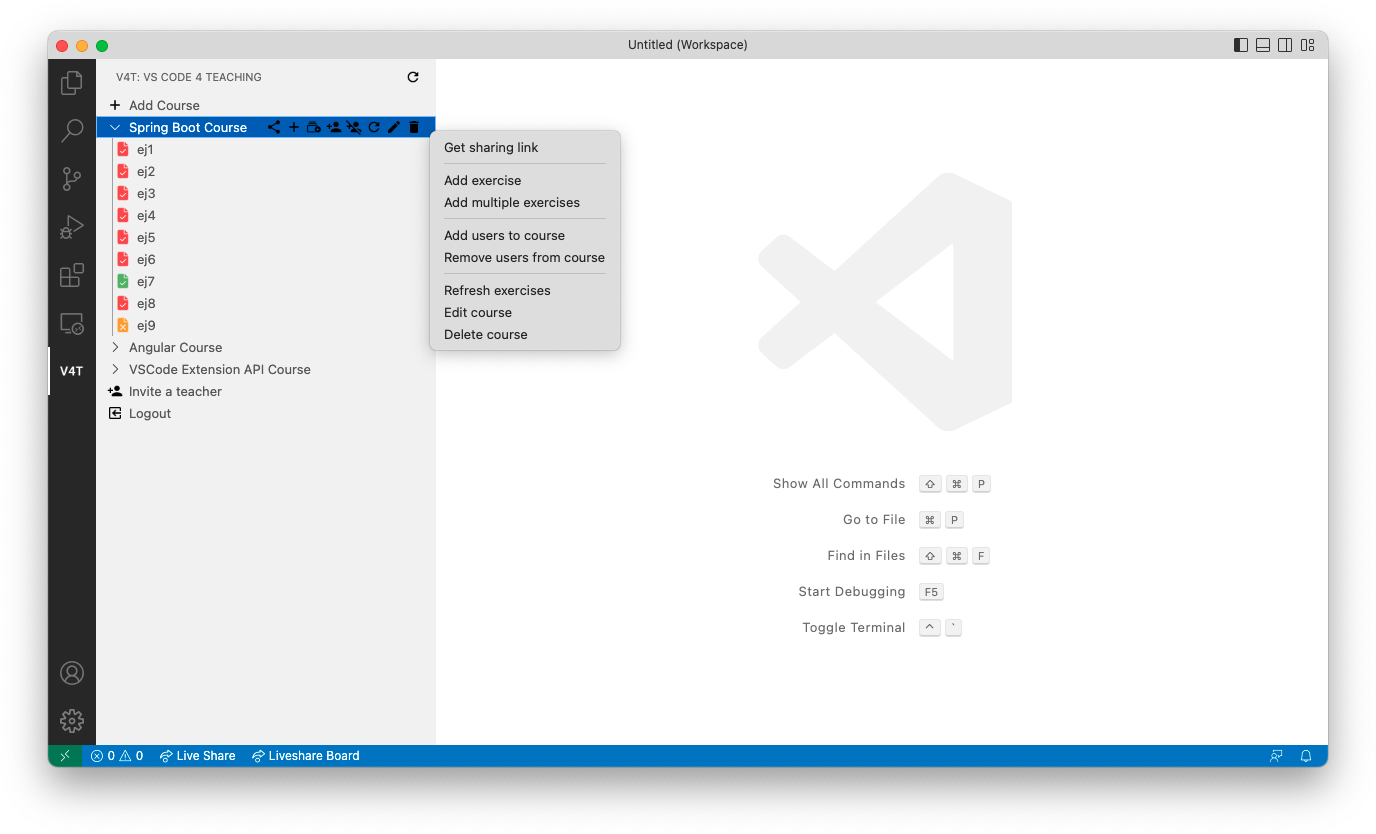
\includegraphics[width=\textwidth]{imagenes/utilizadas/4-3-implementacion/rf10-1.png}
    \caption{Menú mostrado a los docentes al hacer \textit{click} secundario sobre un curso.}
    \label{fig:reqf10-1}
\end{figure}
